% Introduction, problem formulation and notation.

\section{Introduction}\label{sec:intro}

Holographic optical tweezers shape one laser beam into many traps with a phase-only spatial light modulator (SLM) placed in the pupil of a lens. The largest published neutral-atom tweezer array holds \execAtoms{} atoms in about \execTweezers{} tweezers, with a trap-depth spread of \execSpread{} percent across its sites~\cite{manetsch}. The spread matters because sites with unequal depth differ in loading probability, in gate fidelity and in imaging, and the light that forms them is hard to keep uniform as the array grows; the same article names the light field as one of the limits of the scale. A small calibrated array reached a much smaller spread~\cite{ultraprecise}, which suggests that the spread is not a fixed limit but depends on how the hologram is computed and on how the device realises it; the two arrays differ in size and set-up, so the comparison is not a controlled one and neither citation shows the cause. Quantum-computing programs pull the array size up: continuous operation of a coherent array of three thousand atoms~\cite{continuous3000} and a logical processor on reconfigurable atom arrays~\cite{logical} depend on arrays that are loaded, rearranged and refreshed many times, and learned holography has been used to assemble defect-free arrays within a constant time~\cite{airearr}. Camera feedback closes the loop on a real set-up and reaches a non-uniformity of about one percent in arrays of more than a thousand spots~\cite{feedbackeq}, at the cost of a camera path and iterations for every array. The calibration of the SLM itself, the wavefront and the pixel crosstalk, is becoming a model-based step that takes minutes~\cite{slmcal}.

The same computation serves other users with different limits. Single-molecule biophysics laboratories use optical tweezers as the method of choice for single-molecule manipulation~\cite{tweezerbio}, and parallel traps help them only when the traps exert equal force; neuroscience groups stimulate ensembles of neurons with holographic patterns, where heating and the intensity that falls far from the zero order bound the light~\cite{neuralens}; laser micro-processing splits one beam into many with a spatial light modulator, with about half of the light in the first-order beams~\cite{machining}; and near-eye display research has developed camera-in-the-loop training of holograms that overlaps with the methods here~\cite{neuralholo}. What the users share is a decision that is taken before any experiment: which method to use to compute the phase, with which device model, and at what cost in time and light.

The hologram methods that answer this decision span half a century: the superposition of prisms and lenses, random superposition and random masks, the Gerchberg--Saxton (GS) iteration and its adaptive and weighted forms~\cite{dileonardo}, direct search~\cite{polin}, conjugate-gradient minimization~\cite{harte}, phase-fixed weighted GS for large arrays~\cite{kim2019}, mixed-region amplitude freedom for shaped potentials~\cite{pasienski}, gradient descent through differentiable forward models~\cite{chakra}, optimal-transport initialization~\cite{swan,torchylo} and learned holography~\cite{eybposh}. A search of the literature found no controlled published comparison of weighted GS, phase-fixed weighted GS, conjugate gradient, MRAF and a learned method on the same point-trap array, and no public tool that runs them side by side with a device model and the physics of what is trapped.

DinHot provides that comparison. It began at CEFOP, Universidad de Concepci\'on, as DinHotSys, a C++ desktop tool for dynamic holographic optical tweezers dated 2010; it was rewritten in Python and FastAPI and is rebuilt here as a static browser application whose numbers are computed by the engine or baked offline and replayed. The studio runs \nLadder{} methods (\nPublished{} published ones and \nProposed{} proposed here) on \nCases{} cases, with the same seeds, metrics and device model, in Python as the reference and in a TypeScript port that runs live in the browser.

\textbf{Contributions.} The report makes the following contributions.
\begin{itemize}
\item A scalar Fourier model of the SLM, the lens and the device (quantization, pixel crosstalk, pixel aperture and flicker) with closed-form adjoints, so that every gradient method differentiates through the device without automatic differentiation (Sections~\ref{sec:problem} and~\ref{sec:methods}).
\item Twenty-four hologram methods implemented behind one interface, nineteen of them replicated from the literature and five proposed here, each with a stated acceptance criterion and a test that measures it (Section~\ref{sec:methods}, Table~\ref{tab:ladder}).
\item Twelve data contracts with schemas, examples, producer and consumer tests and a declared behaviour for missing data (Section~\ref{sec:data}).
\item A benchmark protocol of \benchRows{} rows over \benchGeometries{} geometries, the ideal device and the device of case C08, every budget of the protocol and up to \benchSeeds{} seeds, and the measured results of the \nCases{} cases (Sections~\ref{sec:protocol} and~\ref{sec:results}).
\item Two learned models trained offline and evaluated on held-out sets written before training: one that beats its baseline at equal wall-clock, and one that is refuted by a control (Section~\ref{sec:learned}).
\item Measured findings that differ from the sources they replicate, each kept as a result: the source value of the freeze index of phase-fixed weighted GS stalls on a crowded array of this grid, and the reconstruction of the adaptive form needs a scale convention (Sections~\ref{sec:m07} and~\ref{sec:m05}).
\end{itemize}

\textbf{Structure.} Section~\ref{sec:problem} states the problem and the models; Section~\ref{sec:notation} collects the notation; Section~\ref{sec:data} documents the cases and the contracts; Section~\ref{sec:architecture} describes the pipeline, the engine and the lanes; Section~\ref{sec:methods} describes the methods one by one; Sections~\ref{sec:protocol} to~\ref{sec:validation} give the protocol, the results and the validation; Sections~\ref{sec:discussion} to~\ref{sec:conclusions} discuss, bound and conclude. Every number in the tables and the text is generated from the committed artifacts of the repository or measured by the scripts kept with this report; the browser timings are quoted from the product's record of measured resources, and the executive figures of this introduction are taken from the cited publications and not re-measured.

\begin{figure}[t]
\centering
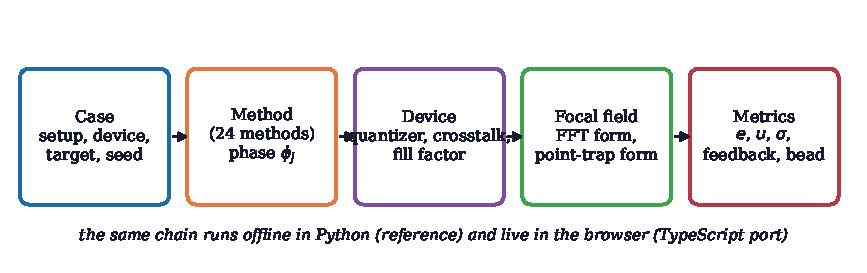
\includegraphics[width=0.95\textwidth]{fig-pipeline.pdf}
\caption{The chain every case runs: a case (optical setup, device, target and seed) is given to a method, which returns a phase; the device model turns the phase into the field the instrument forms; the metrics score the traps, and the feedback and particle simulations act on the scored field.}
\label{fig:pipeline}
\end{figure}

\section{Problem formulation}\label{sec:problem}

\subsection{Inputs, outputs and variables}\label{sec:problem-io}

The problem is posed per case, and every case runs the chain of Figure~\ref{fig:pipeline}. A case fixes an optical setup, a device, a target, an aberration, a set of methods and budgets, and a seed. The optical setup is the vacuum wavelength $\lambda$, the focal length $f$ of the lens, the numerical aperture $\mathrm{NA}$, the immersion index $n_{\mathrm{imm}}$ and the input beam, a Gaussian whose intensity is $\exp(-2r^2/w_{\mathrm b}^2)$ with waist $w_{\mathrm b}=w_{\mathrm{frac}}\,n_{\mathrm{pix}}\,p/2$, normalised so that $\sum_jA_j^2=N_{\mathrm{pix}}$. The device is the SLM: $n_{\mathrm{pix}}\times n_{\mathrm{pix}}$ pixels of pitch $p$, a phase resolution of $b$ bits, a fill factor, a crosstalk kernel and a flicker amplitude. The target is either a list of traps, each with a position $(x_m,y_m,z_m)$, a relative weight $w_m$ and a vortex charge $l_m$, or a shaped potential given as an amplitude and a signal mask on the focal grid. The aberration is a set of Zernike coefficients in waves, and the seed fixes every random draw of the run. The output of a method is a phase $\phi_j\in[0,2\pi)$ for every pixel $j$ at position $(x_j,y_j)$ from the optical axis, together with the history of the metrics along the iterations. The quantities that the problem estimates are the metrics of the hologram on the device (Section~\ref{sec:problem-obj}) and the dynamics of what is trapped (Section~\ref{sec:problem-trap}).

Table~\ref{tab:notation} lists the symbols and their units. Lengths on the focal plane are carried in micrometres and in Fourier units, one unit being the width $\lambda f/(n_{\mathrm{pix}}p)$ of a bin of the unpadded transform, so that a trap on an integer multiple of a bin has a closed form in both models. A trap is refused if its position lies at or beyond the unaliased half field of Eq.~\eqref{eq:window}, which is the rule that case C11 exists to prove.

\subsection{Forward model, objective and constraints}\label{sec:problem-obj}

For a trap $m$ at $(x_m,y_m,z_m)$ with vortex charge $l_m$, the phase delay from SLM pixel $j$ is
\begin{equation}
\Delta_j^m=\frac{\pi z_m}{\lambda f^2}(x_j^2+y_j^2)+\frac{2\pi}{\lambda f}(x_jx_m+y_jy_m)+l_m\operatorname{atan2}(y_j,x_j),
\label{eq:delay}
\end{equation}
and the field and the intensity of trap $m$ are
\begin{equation}
V_m=\frac1{N_{\mathrm{pix}}}\sum_jA_je^{\,i(\phi_j-\Delta_j^m)},\qquad I_m=|V_m|^2,
\label{eq:field}
\end{equation}
following Di Leonardo et al.~\cite{dileonardo}, so that $I_m$ is the fraction of the input power in the peak of trap $m$. The second form of the model is the centred, zero-padded, orthonormal fast Fourier transform of the SLM field; at a trap on a bin with $z=0$ and no vortex the two forms agree exactly, $V_m=E[\mathrm{bin}]\,\mathrm{pad}/n_{\mathrm{pix}}$, which the test suite checks. One bin of the padded transform and the half-window that the pixel sampling leaves unaliased are
\begin{equation}
\Delta x=\frac{\lambda f}{\mathrm{pad}\,n_{\mathrm{pix}}\,p},\qquad X_{1/2}=\frac{\lambda f}{2p},
\label{eq:window}
\end{equation}
and the grid spans the replica period $\lambda f/p$ of the pixel sampling, so that replicas fold onto it and are counted as ghosts in the power budget. Depth is handled by the angular spectrum with the evanescent components removed,
\begin{equation}
H=\exp\!\Big(2\pi i\frac{\Delta z}{\lambda_m}\sqrt{1-(\lambda_m\xi_x)^2-(\lambda_m\xi_y)^2}\Big),\qquad \xi_x^2+\xi_y^2<\lambda_m^{-2},\quad\lambda_m=\frac{\lambda}{n_{\mathrm{imm}}},
\label{eq:angspec}
\end{equation}
which assumes the scalar paraxial model, so that the axial position of a displaced trap is exact only for $|z|\ll f$.

With $I_m$ the trap intensities (divided by the target weights where they differ) the problem is scored by three metrics,
\begin{equation}
e=\sum_mI_m,\qquad u=1-\frac{\max I-\min I}{\max I+\min I},\qquad \sigma=100\,\frac{\operatorname{std}(I)}{\operatorname{mean}(I)}\ \text{percent},
\label{eq:metrics}
\end{equation}
the efficiency, the uniformity ($u=1$ is perfect) and the relative standard deviation, the last with the population standard deviation. Polin et al.~\cite{polin} use the same ratio without the leading one, a non-uniformity; the two are never mixed here. A power budget separates the traps, the zero order, the ghost traps (everything else on the grid, including folded replicas) and the remainder, which Parseval's relation makes zero for the plain Fourier form. The problem is a multi-criteria one: maximize $e$ and $u$ together (and minimize $\sigma$), over the phase $\phi$, subject to the constraints that the phase is realisable by the device, that the traps lie inside the unaliased field, and that the input beam has the stated, not necessarily flat, amplitude. The last constraint bounds the efficiency. For one trap the bound follows from Eq.~\eqref{eq:field}, since $|V_m|\le\overline A$; for the metric of the engine the record of the forward model states the ceiling for a Gaussian input beam as
\begin{equation}
e\le(\overline A)^2,\qquad \overline A=\frac1{N_{\mathrm{pix}}}\sum_jA_j,
\label{eq:ceiling}
\end{equation}
which is \refLevel{} at the test setup. The bound holds for one trap: $|V_m|\le\overline A$, with equality for the phase that puts all the terms of Eq.~\eqref{eq:field} in phase, and $\overline A^2\le1$ by the Cauchy--Schwarz inequality, with equality for a flat beam. For many traps on distinct Fourier units the traps are orthogonal channels of a unit-norm pupil field, and the only bound that holds for every beam and every phase is $e\le1$ (Bessel's inequality); $\overline A^2$ is not a bound there. A numerical maximization of the sum of the trap intensities over all pixel phases for the Gaussian beam of the test setup (\texttt{data/ceiling\_check.py}: Adam, 600 iterations, one seed, the closed-form adjoint of the engine) gives $e=\ceilTwoBins$ for ten traps one Fourier unit apart, above the reference level \refLevel{}, while ten traps eight bins apart reach $\ceilEightBins$, the level itself, and a $10\times10$ lattice at the same spacing reaches $\ceilLattice$ in the same budget, below it. These are measurements on one setup and one seed and not a proof, and they depend on the spacing; traps on adjacent bins of the padded grid are not orthogonal channels, and the same check gives $\ceilAdjacent$ for them, above one, so that Bessel's bound does not apply to them. The value $\overline A^2$ is used in this report only as the reference level of the single-trap limit, and the acceptance criteria that state a fraction of it are thresholds against that reference, not against a proven ceiling. For a shaped potential the metrics are the signal-region ones: the fraction of the power in the signal region, and the root-mean-square fractional error $\eta$ of Eq.~\eqref{eq:m08-err} over the measure region.

\subsection{The device and what is trapped}\label{sec:problem-trap}

A real SLM quantizes the phase, couples neighbouring pixels, covers only part of each pixel and fluctuates. The device model applies, in order, wrapping, quantization to $2^b$ levels, a nonlinear response $2\pi(\phi_q/2\pi)^{\gamma}$, Gaussian flicker of stated rms and wrapping, and blurs the upsampled phase with the crosstalk kernel of Eq.~\eqref{eq:m13}, whose fitted parameters $\sigma_K=\devcXtSigma$ and $q=\devcXtQ$ on $3\times3$ sub-pixels are those of Schroff et al.~\cite{schroff} (an error below two percent in that work). A square pixel of fill factor $\mathrm{fill}$ multiplies the focal field by a product of cardinal sines, so that the intensity envelope and the first-order efficiency of a stepped grating with $N$ levels are
\begin{equation}
\mathcal E(x)=\operatorname{sinc}^2\!\Big(\frac{\sqrt{\mathrm{fill}}}{2}\,\frac{x}{X_{1/2}}\Big),\qquad \eta_1=\operatorname{sinc}^2\!\Big(\frac1N\Big),
\label{eq:envelope}
\end{equation}
so that the intensity falls to about 0.4 at the edge of the unaliased window; the envelope is derived in the engine and tested against a brute-force transform, and the stepped-grating efficiency is a published result~\cite{moreno} (Figure~\ref{fig:device} shows both, and the kernel). Flicker is a computed parameter: the one measured device that was read is a twisted-nematic display with a large fluctuation~\cite{lizana}, so the flicker of case C08 is a stated parameter and not a calibrated one. Zernike aberrations are expanded in the Zernike polynomials of Noll~\cite{noll}, with the single-index ordering of the engine (Section~\ref{sec:m14}), and enter as an additive wavefront on the SLM phase.

\begin{figure}[t]
\centering
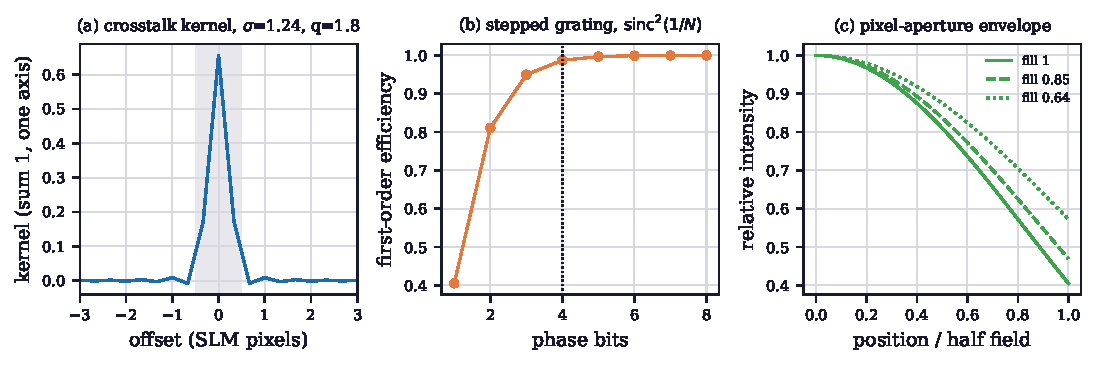
\includegraphics[width=\textwidth]{fig-device.pdf}
\caption{The device model at the parameters of case C08: (a) the crosstalk kernel along one axis, the inverse transform of Eq.~\eqref{eq:m13} on the sub-pixel grid, with the width of one SLM pixel shaded; (b) the first-order efficiency of a stepped grating against the number of phase bits, with the C08 resolution dotted; (c) the pixel-aperture envelope of Eq.~\eqref{eq:envelope} across the unaliased half field, for fill factors of one, the C08 value and 0.64.}
\label{fig:device}
\end{figure}

What is trapped follows from the intensity. For an atom in a red-detuned beam the dipole potential and the radial and axial trap frequencies of a focused Gaussian are, after Grimm, Weidem\"uller and Ovchinnikov~\cite{grimm},
\begin{equation}
U_{\mathrm{dip}}=\frac{3\pi c^2}{2\omega_0^3}\frac{\Gamma}{\Delta}\,I,\qquad \omega_r=\sqrt{\frac{4\hat U}{mw_0^2}},\qquad \omega_z=\sqrt{\frac{2\hat U}{mz_R^2}},
\label{eq:atom}
\end{equation}
with $\hat U$ the trap depth, $w_0$ the waist and $z_R=\pi w_0^2/\lambda$ the Rayleigh range of the focus. For a Rayleigh bead the gradient force gives a stiffness proportional to the intensity curvature~\cite{bouloumis},
\begin{equation}
\kappa_i=-\frac{\operatorname{Re}(\alpha)}{2n_mc\epsilon_0}\frac{\partial^2I}{\partial x_i^2},\qquad f_c=\frac{\kappa}{2\pi\gamma},\qquad P(f)=\frac{D}{\pi^2(f^2+f_c^2)}\quad(f>0),
\label{eq:bead}
\end{equation}
where $\alpha$ is the polarizability, $\gamma$ the Stokes drag, $D=k_BT/\gamma$ the diffusion coefficient and $P(f)$ the thermal Lorentzian spectrum of a trapped bead, from which the stiffness is calibrated~\cite{tolic}. The convention is the one-sided spectrum on $f>0$, which is the form the engine fits to the simulated trace; the two-sided spectrum on $-\infty<f<\infty$ has half that value, $D/[2\pi^2(f^2+f_c^2)]$. For a sphere of radius $r$ and index $n_p$ in a medium of index $n_m$ the polarizability is $\alpha=4\pi\epsilon_0n_m^2r^3(m^2-1)/(m^2+2)$ with $m=n_p/n_m$, and $I=\frac12n_mc\epsilon_0|E|^2$ is the intensity in the medium, so the gradient force is $\mathbf F=\frac{2\pi n_mr^3}{c}\frac{m^2-1}{m^2+2}\nabla I$, derived here from the polarizability above (Harada and Asakura~\cite{harada} treat the radiation forces on a dielectric sphere in the Rayleigh regime; their printed equation was not checked); the dipole force of Bouloumis and Nic Chormaic~\cite{bouloumis} (their Eq.~9) is its vacuum case, $n_m=1$. A bead with $n_p<n_m$ has a negative polarizability and is pushed out of the focus.

\subsection{Assumptions and where each comes from}\label{sec:problem-assume}

The model is scalar and paraxial: the engine computes Fraunhofer and angular-spectrum propagation, and a high numerical aperture is flagged as outside its validity (case C07) because the vectorial equations of the focus were not read at the source. The cases are synthetic: the optical setups, devices and targets are stated parameters taken from published experiments, labelled as such, and no measured sample is used. Absolute numbers therefore belong to the stated model and not to a measured instrument. The device parameters of the crosstalk kernel come from a published fit, while the fill-factor, four-bit and flicker effects have no published source in this build and are computed only; the pixel that the kernel width refers to (SLM or computational pixel, a factor of three) is the engine's reading and is not settled by the source (Section~\ref{sec:m13}). The emulated camera has errors that are stated parameters. The input beam is a Gaussian of stated waist unless a test uses a flat beam. The randomness is the portable generator of the engine, so that every run is a pure function of its parameters and its seed. Each of these assumptions bounds a claim in Section~\ref{sec:limitations}.

\section{Notation}\label{sec:notation}

\begin{table}[t]\centering\footnotesize
\caption{Notation: every symbol of the report with its meaning and its unit; a unit of 1 marks a dimensionless quantity or a count, and the intensities are fractions of the input power.}\label{tab:notation}
\begin{tabular}{@{}>{\raggedright\arraybackslash}p{0.2\textwidth} >{\raggedright\arraybackslash}p{0.56\textwidth} >{\raggedright\arraybackslash}p{0.16\textwidth}@{}}\toprule Symbol & Meaning & Unit\\\midrule
$\lambda$ & vacuum wavelength of the laser & nm\\
$f$ & focal length of the lens in the pupil of which the SLM sits & mm\\
$\mathrm{NA}$ & numerical aperture of the objective & 1\\
$n_{\mathrm{imm}}$ & refractive index of the immersion medium & 1\\
$n_{\mathrm{pix}}$ & SLM pixels per side & 1\\
$N_{\mathrm{pix}}$ & number of SLM pixels, $n_{\mathrm{pix}}^2$ & 1\\
$p$ & SLM pixel pitch & $\mu$m\\
$\mathrm{pad}$ & zero-padding factor of the focal grid & 1\\
$n_{\mathrm{fft}}$ & focal grid size, $\mathrm{pad}\,n_{\mathrm{pix}}$ & 1\\
$j$ & index of an SLM pixel, at position $(x_j,y_j)$ from the optical axis & m\\
$m,\ M$ & index and number of traps & 1\\
$(x_m,y_m,z_m)$ & position of trap $m$ in the focal volume & $\mu$m\\
$l_m$ & vortex (topological) charge of trap $m$ & 1\\
$w_m,\ a_m$ & target weight of trap $m$ and its target amplitude $\sqrt{w_m}$ & 1\\
$A_j$ & input beam amplitude, normalised so that $\sum_jA_j^2=N_{\mathrm{pix}}$ & 1\\
$\phi_j$ & phase displayed at pixel $j$ & rad\\
$\Delta_j^m$ & phase delay from pixel $j$ to trap $m$ (Eq.~\eqref{eq:delay}) & rad\\
$V_m,\ I_m$ & complex field at trap $m$ and its intensity $|V_m|^2$ (fraction of the input power) & 1\\
$e$ & efficiency, the sum of the trap intensities & 1\\
$u$ & uniformity, $1-(\max I-\min I)/(\max I+\min I)$ & 1\\
$\sigma$ & relative standard deviation of the trap intensities & percent\\
$\eta$ & root-mean-square fractional error of a shaped potential in its measure region & 1\\
$\Delta x,\ X_{1/2}$ & width of one focal bin and half of the unaliased field & $\mu$m\\
$K,\ \sigma_K,\ q$ & crosstalk kernel of the device and its fitted width and exponent & 1\\
$Z_j,\ c_j$ & Zernike mode $j$ (Noll order) and its coefficient & waves\\
$N$ (or $n_{\mathrm{fix}}$) & iteration after which the focal phase is frozen & 1\\
$\alpha$ & exponent of the assignment cost (M16) or weight of the adaptive form (M05) & 1\\
$m$ (mixing) & mixing parameter of the mixed-region rule & 1\\
$G,\ \rho_m$ & feedback gain and measured intensity relative to its target & 1\\
$\lambda_{\mathrm{B5}}$ & trade-off parameter of the front & 1\\
$\mathrm{AC}$ & accuracy of a volume hologram, mean over planes of the overlap of unit-sum intensities & 1\\
$z_R$ & SLM-limited Rayleigh range & mm\\
$\kappa,\ \gamma,\ f_c$ & trap stiffness, drag coefficient and corner frequency of a bead & pN/$\mu$m, kg/s, Hz\\
$U,\ \omega_r$ & dipole potential depth of an atom and its radial trap frequency & J, rad/s\\
\bottomrule\end{tabular}\end{table}


Table~\ref{tab:notation} fixes the symbols that are used in more than one section. Three conventions apply throughout. First, indices: $j$ runs over SLM pixels and $m$ over traps, the iteration is a superscript $k$ or a subscript $i$ where the source of the method uses it, and the focal bins carry the coordinate $\mathbf u$ of the padded transform. Second, normalisation: every intensity $I_m$ is a fraction of the input power, so that the efficiency $e$ lies between zero and one (the single-trap reference level of Eq.~\eqref{eq:ceiling} is not a bound for many traps); the relative standard deviation is carried in percent and never as a fraction, which the units gate of Section~\ref{sec:validation} checks on every shipped artifact; and phases are in radians, with the Zernike coefficients in waves and the unit-rms basis so that the rms of the wavefront is the root sum of squares of the coefficients. Third, units: positions are in micrometres on the focal plane and in metres in the engine's internal interface, the pixel pitch in micrometres, the wavelength in nanometres, the focal length in millimetres, times in seconds and frequencies in hertz; a position in metres where micrometres are expected would be about a hundred thousand times too small, which the same gate catches. The ids M01 to M19 and B1 to B5 are the engine's compact labels for the methods, kept in tables, while the text names each method; a method id is a label and not a ranking.

The objects that carry the notation in the code are the setup of the optical system, the target (traps or a shaped field with its signal mask), the budget (an iteration cap and an optional wall-clock cap), the result (the phase, the history, the trap fields and a metadata record) and the method specification (identifier, name, family, lane, supported targets and dimensions). The interface is documented in Section~\ref{sec:arch-engine}. Where a symbol is overloaded by the sources, the report keeps the source's symbol in the method section where it is used and states the mapping: for example the exponent $\alpha$ of the assignment cost of Eq.~\eqref{eq:m16} and the weight $\alpha$ of Eq.~\eqref{eq:m05} are different quantities, and the mixing $m$ of Eq.~\eqref{eq:m08} is not the trap index. The overloads that remain are these. The polarizability $\alpha$ of Eq.~\eqref{eq:bead} is a third $\alpha$; the index ratio $m=n_p/n_m$ of the polarizability and the atomic mass $m$ of the trap frequencies of Eq.~\eqref{eq:atom} are two more $m$. The width $w_{\mathrm b}$ of the input beam is not the trap weight $w_m$, and the waist and Rayleigh range of the focus of an atom, $w_0$ and $z_R$, are not the SLM-limited range $z_{R,\mathrm{SLM}}$ of the volume network. The focal length $f$ of the lens is not the frequency $f$ of the bead spectrum nor the weight $f_u$ of the direct-search cost. The relative standard deviation $\sigma$ of Eq.~\eqref{eq:metrics} is in percent, whereas the kernel width $\sigma_K$ and the residual $\sigma$ of the direct-search cost are not; $\gamma$ is the Stokes drag of the bead, the best scale of the direct-search cost and the coefficient of the conjugate-gradient direction in the three places where each is defined; and $\eta$ is the error of a shaped potential, the first-order efficiency $\eta_1$ of a stepped grating and the efficiency level that the optimizers request, each defined where it is used.
